\documentclass[a4paper,12pt]{article}

\usepackage[T1]{fontenc}
\usepackage{amsmath}
\usepackage{amssymb}

\usepackage[margin=2cm]{geometry}

\usepackage{graphicx}
\usepackage{xcolor}  

\usepackage[bottom]{footmisc}     
\usepackage{caption}

\usepackage{url}
\usepackage[bookmarksnumbered,breaklinks]{hyperref}
\usepackage{breakurl}

\usepackage{listings}

\colorlet{punct}{red!60!black}
\definecolor{background}{HTML}{EEEEEE}
\definecolor{delim}{RGB}{20,105,176}
\colorlet{numb}{magenta!60!black}

\lstdefinelanguage{json}{
    basicstyle=\normalfont\ttfamily,
%    numbers=left,
    numberstyle=\scriptsize,
    stepnumber=1,
    numbersep=8pt,
    showstringspaces=false,
    breaklines=true,
%    frame=lines,
    backgroundcolor=\color{background},
    literate=
     *{0}{{{\color{numb}0}}}{1}
      {1}{{{\color{numb}1}}}{1}
      {2}{{{\color{numb}2}}}{1}
      {3}{{{\color{numb}3}}}{1}
      {4}{{{\color{numb}4}}}{1}
      {5}{{{\color{numb}5}}}{1}
      {6}{{{\color{numb}6}}}{1}
      {7}{{{\color{numb}7}}}{1}
      {8}{{{\color{numb}8}}}{1}
      {9}{{{\color{numb}9}}}{1}
      {:}{{{\color{punct}{:}}}}{1}
      {,}{{{\color{punct}{,}}}}{1}
      {\{}{{{\color{delim}{\{}}}}{1}
      {\}}{{{\color{delim}{\}}}}}{1}
      {[}{{{\color{delim}{[}}}}{1}
      {]}{{{\color{delim}{]}}}}{1},
}


\newcommand{\angstrom}{\textup{\AA}}

\begin{document}
\title{Schroedinger--Poisson solver for 2D materials:\\documentation}
\date{\today}
\author{Augustin Bussy \and Giovanni Pizzi \and Marco Gibertini} 
\maketitle

\section{Introduction}

This code aims at self-consistently solving the coupled Schr\"odinger--Poisson equations in 2D materials. More precisely, in the current implementation it is designed to simulate nanosheets of a single material with regions of different strains. The Schr\"odinger equation is in 1D, meaning that the strain can vary on a single axis ($x$), as illustrated in Fig.~\ref{fig:example1}. Moreover, the material is assumed to be infinite in the $y$ direction and periodic in the $x$ direction.

Two types of calculations can be performed: \emph{single-point} or \emph{map}. The former (\emph{single-point}) simulates a specific setup as described in an input file provided by the user (see Sec.~\ref{sec:input}) to produce a band profile and/or a carrier density profile. This is a useful tool for experiments as it allows to simulate any strain profile. The \emph{map} calculation type, instead, screens over different setups of strained/unstrained material to investigate, e.g., metal-insulator phase transitions.

This code uses a multi-scale approach, meaning that the materials properties must be provided as input, typically calculated from DFT calculations. These quantities include effective masses and polarization charges for different strains. The properties for at least 4 or 5 strains should be provided for accurate fitting. It is also not recommended to extrapolate strains larger than those coming from DFT, as the trends could change.

\begin{figure} [h]
\begin{center}
\captionsetup{width=0.95\textwidth}
\centerline{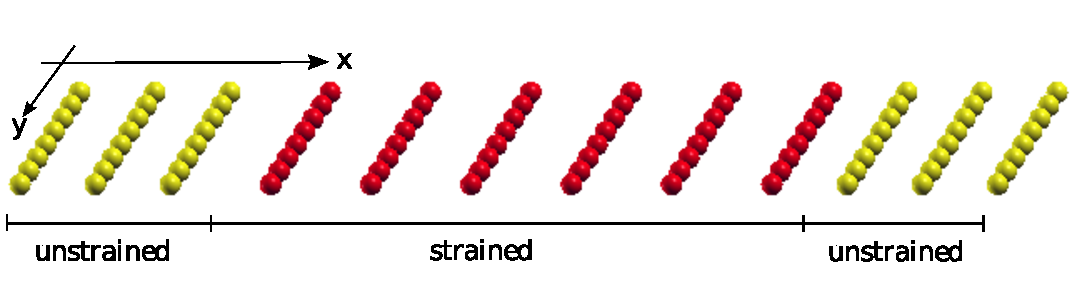
\includegraphics[width=12cm,angle=0]{img/example1}}
\caption{\small Example of simulation setup: periodic alternation of strained and unstrained regions of a given material.}
\label{fig:example1} 
\end{center}
\end{figure}

\section{How to cite}
If you use this code in your work, please cite the following paper: \\
A. Bussy, G. Pizzi, M. Gibertini, \emph{Strain-induced polar discontinuities in 2D materials from combined first-principles and Schr\"odinger-Poisson simulations}, \underline{\href{http://arxiv.org/abs/1705.01303}{arXiv:1705.01303}} (2017).

\section{Compiling and running up the code}
The code is distributed in the \texttt{code} folder, and consists of three main files.
The bulk of the numerical computations is written in Fortran in the  \texttt{schrpoisson\_wire.f90} file. This is interfaced to python using \texttt{f2py}, and the interface has been generated by us in the \texttt{schrpoisson\_wire.pyf} file. (If you decide to modify the name, number or signature of the Fortran functions, you need to regenerate this file. This is possible by running the command commented in the Makefile.)

To compile the code, run the \texttt{make} command in the \texttt{code} folder.
You will need to have the \texttt{f2py} executable\footnote{In most cases, if you already have a recent python distribution and \texttt{pip}, you just need to run \texttt{pip install numpy}, or use your package manager to install python-numpy. See here for more information: \url{https://docs.scipy.org/doc/numpy-dev/f2py/}}, that is part of \texttt{numpy}. 

After running \texttt{make}, the main python code (\texttt{2Dschrpoisson.py}) is ready to be run using the following command:

\begin{quote}
\texttt{python 2Dschrpoisson.py \{material\_properties\}.json  \{calc\_input\}.json}
\end{quote}

Note that if the two input json files are not in the same folder, you need to specify the full path to them.

\section{\label{sec:input}Input}
Two input files are necessary to every calculation: one containing the materials properties and the other the calculation setup. 

\subsection{Material Properties File}
The properties of the material at different strains must be provided in \texttt{json} file as first command line option. 
The file should contain a dictionary, where the key is a string representation of the
float value, and the value should be a dictionary with a given number of keys, as shown in
the example below.

The following example is taken from the \texttt{SnSe\_example.json} file in the \texttt{input\_examples} folder. Note that the properties of the unstrained material are \emph{mandatory} and must be provided under the ``\texttt{0.00}'' key. After the example we provide some explanatory comments.

\subsubsection*{File example}

\begin{lstlisting}[language=json,firstnumber=1]
{"0.00": {
   "alpha_xx": 10.22,
   "x_lat": 4.408,
   "y_lat": 4.288,
   "polarization_charge": 0.0,
   "vacuum_level": 3.471695,
   "valence_gamma": { 
     "energy": -1.508255819,
     "conf_mass": 1.755925079,
     "DOS_mass": 2.7330924,
     "degeneracy": 1
   },
   "valence_gamma-X": {
     "energy": -0.8832657543,
     "conf_mass": 0.125168454,
     "DOS_mass": 0.159070572,
     "degeneracy": 2
   },
   "valence_gamma-Y": {
     "energy": -1.064317364,
     "conf_mass": 0.109554071,
     "DOS_mass": 0.159511425,
     "degeneracy": 2
   },
   "conduction_gamma": {
     "energy": 0.6090962485,
     "conf_mass": 2.741100107,
     "DOS_mass": 2.994158008,
     "degeneracy": 1
   },
   "conduction_gamma-X": {
     "energy": 0.0902128713,
     "conf_mass": 0.110807373,
     "DOS_mass": 0.190387132,
     "degeneracy": 2
   },
   "conduction_gamma-Y": {
     "energy": 0.05720314215,
     "conf_mass": 0.131542031,
     "DOS_mass": 0.130378261,
     "degeneracy": 2
   }
 },
 "0.01": {
   ...
 },
 ...
}
\end{lstlisting}


\subsubsection*{Description of the keys in each subdictionary, for each strain}
\begin{description}
\item[\texttt{alpha\_xx}] Value of the polarizability of the strained material in \angstrom. $x$ is the direction along which different strains/materials alternate (see Fig.~\ref{fig:example1}).

\item[\texttt{x\_lat}, \texttt{y\_lat}] The lattice parameters of the unit cell in \angstrom. \emph{Only needed for the unstrained material.}

\item[\texttt{polarization\_charge}] Polarization charge at the edge of the material in units of electron per unit cell width, \textit{i.e.}, e/$b$.

\item[\texttt{vacuum\_level}] Needed to align energy levels across the setup (in eV).

\item[Energy extrema keys] They need to either contain the string \texttt{valence} or \texttt{conduction} (this is a requirement by the code). The assigned value is a subdictionary with the energy of the band extremum in eV (\texttt{energy}), the confinement mass (\texttt{conf\_mass}) and density of states DOS mass (\texttt{DOS\_mass}) [that are respectively the effective masses in the $x$ and $y$ directions)] and the degeneracy of the energy level in the first BZ (\texttt{degeneracy}).
\end{description}


\subsection{Calculation Input File}
Each type of calculation (single-point or map) has its own input file template with different keys. In both cases, the input file should be in \texttt{json} format and be provided as the second command line argument. 

The following examples can be found in the \texttt{input\_examples} folder. In the same folder, a simple python script (\texttt{create\_calc\_input.py}) could be useful to write a json file starting from a python dictionary.

\subsubsection{Single-point calculation}

\begin{lstlisting}[language=json,firstnumber=1]
  {   
    "calculation": "single_point", 
    "out_dir": "single_point_output", 
    "smearing": true, 
    "KbT": 0.005,
    "max_iteration": 1000, 
    "plot_fit": false, 
    "nb_of_states_per_band": 2, 
    "delta_x": 0.5, 
    "setup": {  
      "slab1": {  
        "polarization": "positive", 
        "strain": 0.0, 
        "width": 15.0
      }, 
      "slab2": { 
        "polarization": "positive", 
        "strain": 0.08, 
        "width": 30.0
      },
      "slab3": { 
        "polarization": "positive", 
        "strain": 0.0, 
        "width": 15.0
      }
    }
  }
\end{lstlisting}

\subsubsection*{Description of the dictionary keys}

\begin{description}
\item[\texttt{calculation}] The value \texttt{"single\_point"} indicates the type of calculation

\item[\texttt{out\_dir}] The name of the folder where the output data is dumped

\item[\texttt{smearing}] If \texttt{true}, a Marzari--Vanderbilt smearing is imposed for the electron distribution. It helps for the convergence of the self-consistent Schroedinger--Poisson loop and allows better comparisons with DFT calculations

\item[\texttt{KbT}] In case of smearing, this is the imposed electronic temperature (Ry)

\item[\texttt{max\_iteration}] The number of allowed steps for the self-consistent Schroedinger--Poisson loop. 1000 is a safe number

\item[\texttt{plot\_fit}] If \texttt{true}, the fitting of materials properties for any strain is displayed interactively in a series of graphs using matplotlib (that needs to be installed)

\item[\texttt{nb\_of\_states\_per\_band}] Useful to limit the size of the output data. In this example, only two quantum states per band (6 in total) will be reported

\item[\texttt{delta\_x}] The size of the discretization step in real space (\angstrom)

\item[\texttt{setup}] The value is a subdictionary with the description of each slab forming the setup. For each layer, one has to specify the \texttt{polarization} (\texttt{positive} or \texttt{negative}: positive if holes accumulate towards larger $x$), the \texttt{strain} of the material and the \texttt{width} of the slab (in \angstrom). There is no limit to the numbers of layers, but the keys must follow the syntax \texttt{slab\%d} where \texttt{\%d} should be replaced with a sequential integer, starting from 1. It is not recommended to include strains larger than those in the material properties file. 

\textbf{Note}: it is also \emph{mandatory} that the first and the last slabs have identical strain, since the code does not cope with polarization charges at the edges of the cell.
\end{description}

\subsubsection{Map calculation}

\begin{lstlisting}[language=json,firstnumber=1]
  { 
    "calculation": "map", 
    "out_dir": "map_output", 
    "smearing": true, 
    "KbT": 0.005, 
    "max_iteration": 1000, 
    "plot_fit": false, 
    "nb_of_steps": 200, 
    "upper_delta_x_limit": 0.5, 
    "strain": {  
      "max_strain": 0.1, 
      "min_strain": 0.0, 
      "strain_step": 0.01
    }, 
    "width": {  
      "min_width": 10.0, 
      "width_step": 5.0, 
      "max_width": 60.0
    }
  }
\end{lstlisting}

\subsubsection*{Description of the dictionary keys}

\begin{description}
\item[\texttt{calculation}] The value \texttt{"map"} indicates the type of calculation

\item[\texttt{out\_dir}] The name of the folder where the output data is dumped

\item[\texttt{smearing}] If \texttt{true}, a Marzari--Vanderbilt smearing is imposed for the electron distribution. It helps for the convergence of the self-consistent Schroedinger--Poisson loop and allows better comparisons with DFT calculations

\item[\texttt{KbT}] In case of smearing, this is the imposed electronic temperature (Ry)

\item[\texttt{max\_iteration}] The number of allowed steps for the self-consistent Schroedinger--Poisson loop. 1000 is a safe number

\item[\texttt{plot\_fit}] If \texttt{true}, the fitting of materials properties for any strain is displayed in a series of graphs using matplotlib (that needs to be installed)

\item[\texttt{nb\_of\_steps}] Since a wide range of setup sizes is spanned in a map calculation, a common step size might be a problem. It is instead dynamically adapted as
$$\Delta x = \frac{L_{tot}}{\text{\texttt{nb\_of\_steps}}}$$

\item[\texttt{upper\_delta\_x\_limit}] In case an (upper) limit should be imposed on the step size: 
$$\Delta x = min\left(\frac{L_{tot}}{\text{\texttt{nb\_of\_steps}}}, 
\text{\texttt{upper\_delta\_x\_limit}}\right)$$

\item[\texttt{strain}] The assigned value is a subdictionary with the lower and upper bound (\texttt{min\_strain} and \texttt{max\_strain}) of the strains over which calculations will be done, as well as the step between strains \texttt{strain\_step}

\item[\texttt{width}] The assigned value is a subdictionary with the lower and upper bound (\texttt{min\_width} and \texttt{max\_width}) of the width over which calculations will be done, as well as the step between widths \texttt{width\_step}. 

\textbf{Note}: the width refers to the unstrained material and the size of the strained slab is computed as $L_{strained} = (1+\epsilon)L_{unstrained}$. 

In this example, 121 single-point calculations will be conducted with every combination of strain $\epsilon = 0.0, 0.01,\ldots,0.1$ and width $L = 10, 15,\ldots, 60$.

\end{description}


\section{Output}

\subsection{Single-Point Calculation}
In single-point calculations, three output files are generated. The first one (\texttt{general\_info.txt}) contains general output information such as the number of iterations needed, convergence parameters and the total free carrier density. The second one (\texttt{band\_data.txt}) contains all the necessary information to produce a band profile (Fermi energy, potential profile of each band, their respective quantum states, etc.).
Finally, the last file (\texttt{density\_profile.txt}) contains the free-electron and free-hole density as a function of position.


\subsection{Map Calculation}
Map calculations produce a single output file in which, among others, the total electron density is given for each strain/width combination. This can be then used to produce a two-dimensional color map.

\end{document}